\documentclass[11pt]{article}
\usepackage{amsmath,amssymb,amsthm}
\usepackage{tikz}
\usetikzlibrary{patterns}

\begin{document}

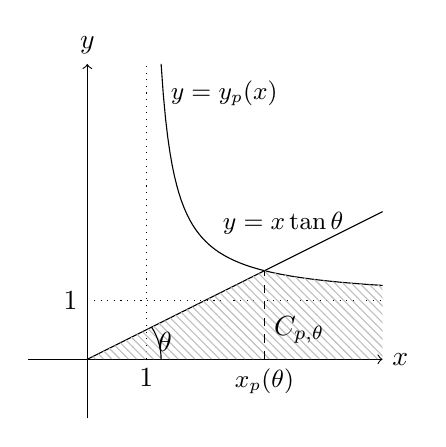
\begin{tikzpicture}[scale=0.75]
\draw[->] (-1,0) -- (5,0);
\draw (5,0) node[right]{$x$};
\draw[->] (0,-1) -- (0,5);
\draw (0,5) node[above]{$y$};
\draw[dotted] (1,0) -- (1,5);
\draw (1,0) node[below]{$1$};
\draw[dotted] (0,1) -- (5,1);
\draw (0,1) node[left]{$1$};
\draw [domain=0:5] plot(\x,{\x/2});
\draw (4.5,2.3) node[left]{\small $y=x\tan\theta$}; %theta vaut plus ou moins 0.5
\draw [domain=1.25:5,samples=100] plot(\x,{1+1/(\x - 1)}); %p vaut 1
\draw (1.25,4.5) node[right]{\small $y=y_p(x)$};
\fill [pattern=north west lines, pattern color=lightgray] (0,0) -- plot [domain=0:3] (\x, \x/2) -- plot [domain=3:5] (\x,{1+1/(\x - 1)}) -- (5,0) -- cycle;
\draw (3,0.5) node[right]{$C_{p,\theta}$};
\draw[dashed] (3,0) -- (3,1.5);
\draw (3,0) node[below]{\small $x_p(\theta)$};
\draw (1.25,0) arc (0:33:1);
\draw (1.6,0.3) node[left]{$\theta$};
\end{tikzpicture}

\end{document}